\documentclass[tikz]{standalone}
\usepackage{tikz}
\usetikzlibrary{decorations.markings}

\begin{document}

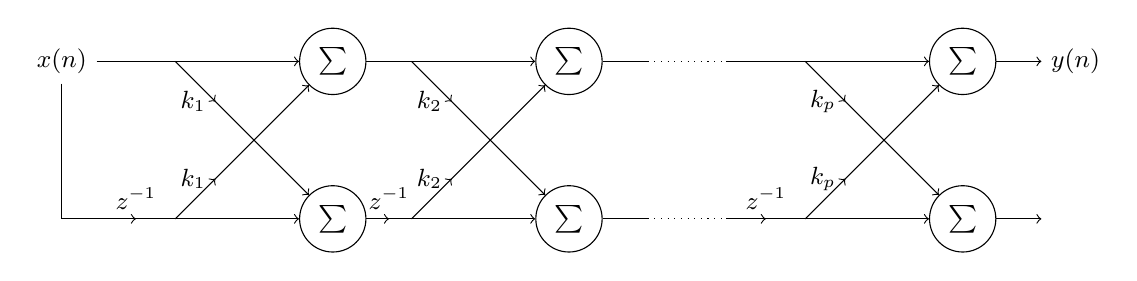
\begin{tikzpicture}[font=\small]
    \tikzset{
        zdelay/.style={
            postaction={decorate},
            decoration={
                markings,
                mark=at position 0.5 with {
                    \arrow{>};
                    \node[above]{$z^{-1}$};
                }
            }
        },
        kgain/.style={
            postaction={decorate},
            decoration={
                markings,
                mark=at position 0.3 with {
                    \arrow{>};
                    \node[left]{#1};
                }
            }
        }
    }

    \coordinate (f0) at (0,0);
    \coordinate (g0) at ([yshift=-2cm] f0);
    \coordinate (f1) at ([xshift=3cm] f0);
    \coordinate (g1) at ([xshift=3cm] g0);
    \coordinate (f2) at ([xshift=3cm] f1);
    \coordinate (g2) at ([xshift=3cm] g1);
    \coordinate (fp1) at ([xshift=2cm] f2);
    \coordinate (gp1) at ([xshift=2cm] g2);
    \coordinate (fp) at ([xshift=3cm] fp1);
    \coordinate (gp) at ([xshift=3cm] gp1);
    \node (x) at ([xshift=-1cm] f0) [left]{$x(n)$};
    \node[circle,draw] (sf1) at ([xshift=2cm] f0) {$\sum$};
    \node[circle,draw] (sg1) at ([xshift=2cm] g0) {$\sum$};
    \node[circle,draw] (sf2) at ([xshift=2cm] f1) {$\sum$};
    \node[circle,draw] (sg2) at ([xshift=2cm] g1) {$\sum$};
    \node[circle,draw] (sfp) at ([xshift=2cm] fp1) {$\sum$};
    \node[circle,draw] (sgp) at ([xshift=2cm] gp1) {$\sum$};
    \node (y) at (fp) [right]{$y(n)$};

    \draw (x) -- (f0);
    \draw (x) |- (g0);
    \draw[->] (f0) -- (sf1);
    \draw[->] (f1) -- (sf2);
    \draw[->] (fp1) -- (sfp);
    \draw[->] (g0) -- (sg1);
    \draw[->] (g1) -- (sg2);
    \draw[->] (gp1) -- (sgp);
    \draw (sf1) -- (f1);
    \draw (sf2) -- (f2);
    \draw[dotted] (f2) -- ([xshift=-1cm] fp1);
    \draw ([xshift=-1cm] fp1) -- (fp1);
    \draw[->] (sfp) -- (fp);
    \draw[zdelay] ([xshift=-1cm] g0) -- (g0);
    \draw[zdelay] (sg1) -- (g1);
    \draw (sg2) -- (g2);
    \draw[dotted] (g2) -- ([xshift=-1cm] gp1);
    \draw[zdelay] ([xshift=-1cm] gp1) -- (gp1);
    \draw[->] (sgp) -- (gp);
    \draw[->,kgain={$k_1$}] (f0) -- (sg1);
    \draw[->,kgain={$k_1$}] (g0) -- (sf1);
    \draw[->,kgain={$k_2$}] (f1) -- (sg2);
    \draw[->,kgain={$k_2$}] (g1) -- (sf2);
    \draw[->,kgain={$k_p$}] (fp1) -- (sgp);
    \draw[->,kgain={$k_p$}] (gp1) -- (sfp);
\end{tikzpicture}

\end{document}